\section{Region Class Reference}
\label{classRegion}\index{Region@{Region}}
{\tt \#include $<$mygraph.h$>$}

Inheritance diagram for Region::\begin{figure}[H]
\begin{center}
\leavevmode
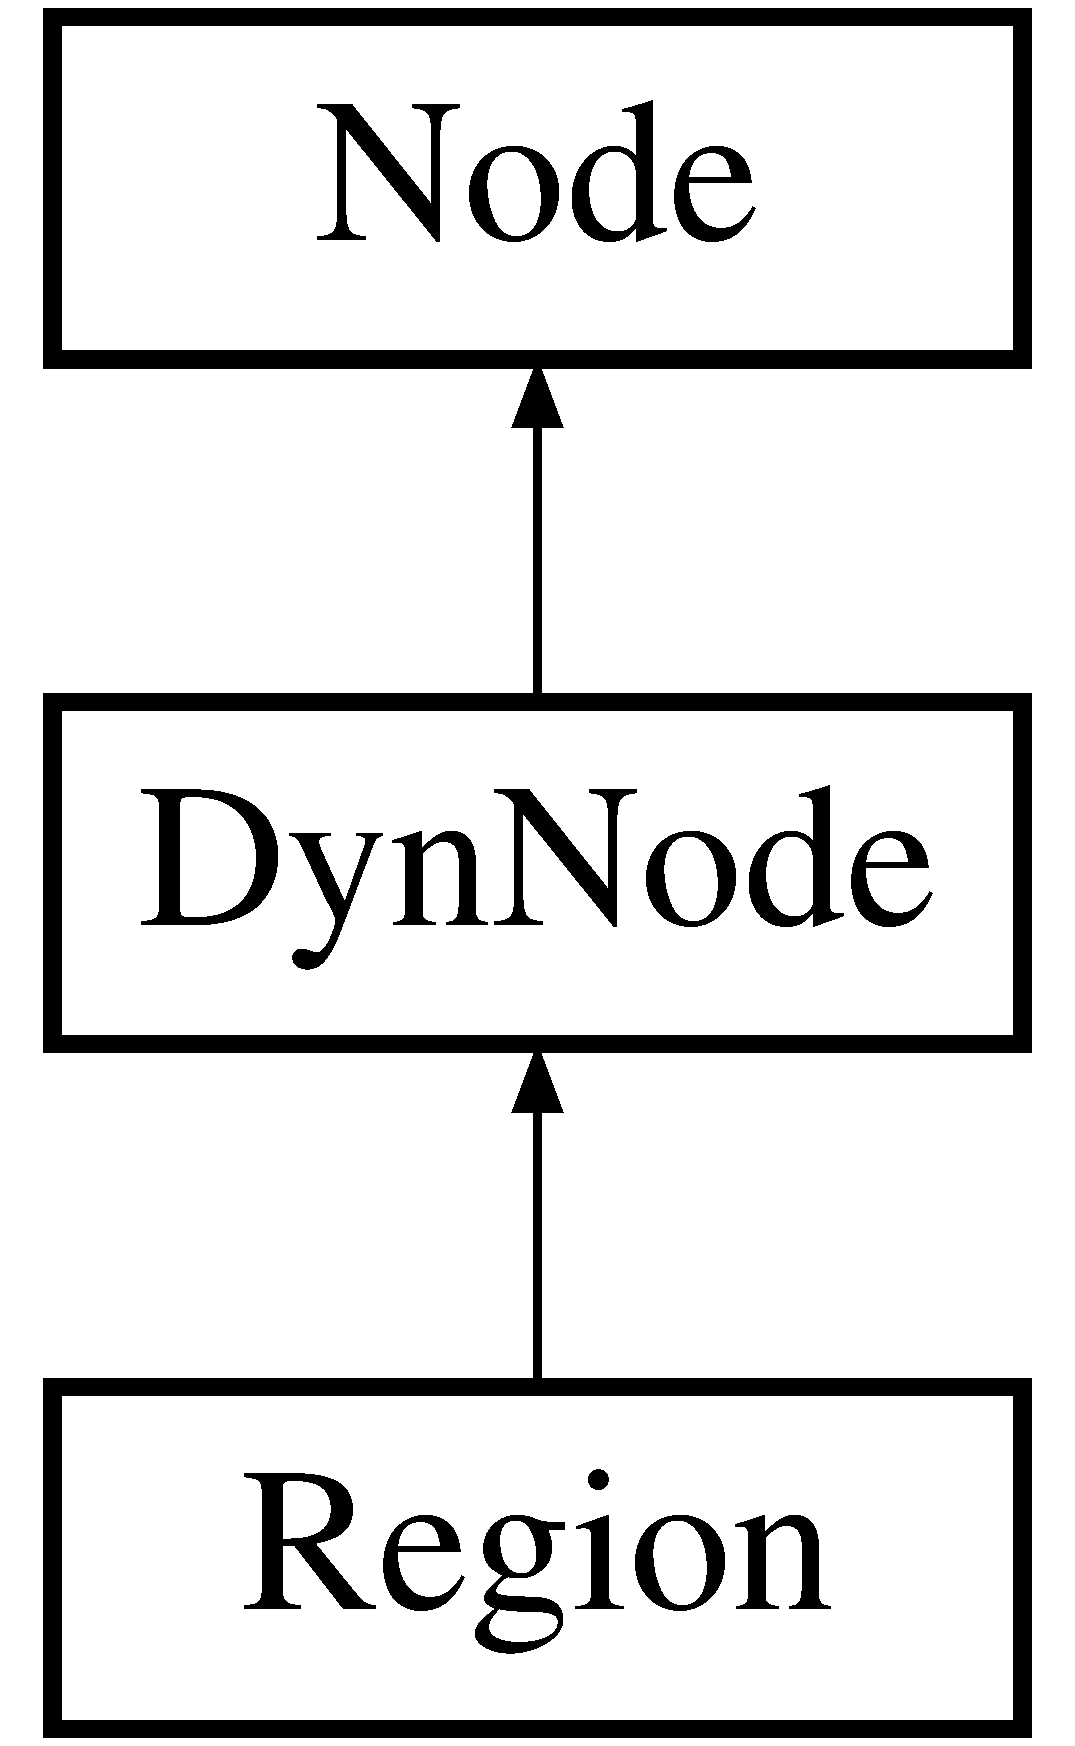
\includegraphics[height=3cm]{classRegion}
\end{center}
\end{figure}
\subsection*{Public Member Functions}
\begin{CompactItemize}
\item 
{\bf Region} ({\bf RegionGraphPtr} \_\-fg, {\bf Cluster} \_\-cl, int \_\-cr, {\bf ConditionalBelief} $\ast$\_\-cb=0)
\item 
{\bf LD} {\bf getStateBlf} (const {\bf StatePtr} sptr) const
\item 
vector$<$ string $>$ {\bf getVarIds} () const
\item 
{\bf LD} {\bf getEntropy} ()
\begin{CompactList}\small\item\em -sum\_\-b b$\ast$log(b) \item\end{CompactList}\item 
{\bf LD} {\bf getEnthalpy} ()
\begin{CompactList}\small\item\em sum\_\-b b$\ast$(-sum\_\-a log f\_\-a) where a is in r \item\end{CompactList}\item 
{\bf LD} {\bf getF} ()
\end{CompactItemize}
\subsection*{Public Attributes}
\begin{CompactItemize}
\item 
int {\bf cr}
\begin{CompactList}\small\item\em counting numbers \item\end{CompactList}\item 
{\bf ConditionalBeliefPtr} {\bf B\_\-t\_\-0}
\begin{CompactList}\small\item\em the K(x0, x\_\-t) factor \item\end{CompactList}\item 
{\bf BeliefPtr} {\bf B\_\-0}
\begin{CompactList}\small\item\em the single ton partition function like function \item\end{CompactList}\item 
{\bf BeliefPtr} {\bf B\_\-t}
\item 
{\bf BeliefPtr} {\bf Z}
\begin{CompactList}\small\item\em the partition function \item\end{CompactList}\end{CompactItemize}
\subsection*{Private Attributes}
\begin{CompactItemize}
\item 
{\bf Cluster} {\bf cl}
\begin{CompactList}\small\item\em the individual factor nodes \item\end{CompactList}\item 
{\bf RegionGraphPtr} {\bf rg}
\item 
{\bf FactorGraphPtr} {\bf fg}
\end{CompactItemize}
\subsection*{Friends}
\begin{CompactItemize}
\item 
ostream \& {\bf operator$<$$<$} (ostream \&os, {\bf Region} \&r)
\end{CompactItemize}


\subsection{Detailed Description}
Implements the region 



\subsection{Constructor \& Destructor Documentation}
\index{Region@{Region}!Region@{Region}}
\index{Region@{Region}!Region@{Region}}
\subsubsection{\setlength{\rightskip}{0pt plus 5cm}Region::Region ({\bf RegionGraphPtr} {\em \_\-fg}, {\bf Cluster} {\em \_\-cl}, int {\em \_\-cr}, {\bf ConditionalBelief} $\ast$ {\em \_\-cb} = {\tt 0})}\label{classRegion_a3c4e2d0fbd5b9337139294ff7db7550}




\subsection{Member Function Documentation}
\index{Region@{Region}!getStateBlf@{getStateBlf}}
\index{getStateBlf@{getStateBlf}!Region@{Region}}
\subsubsection{\setlength{\rightskip}{0pt plus 5cm}{\bf LD} Region::getStateBlf (const {\bf StatePtr} {\em sptr}) const}\label{classRegion_22cb607c718710a6486e7982c1870950}


\index{Region@{Region}!getVarIds@{getVarIds}}
\index{getVarIds@{getVarIds}!Region@{Region}}
\subsubsection{\setlength{\rightskip}{0pt plus 5cm}vector$<$string$>$ Region::getVarIds () const\hspace{0.3cm}{\tt  [inline]}}\label{classRegion_70b5d23ef485e9ead4a2d8ab4e8e6ba7}


\index{Region@{Region}!getEntropy@{getEntropy}}
\index{getEntropy@{getEntropy}!Region@{Region}}
\subsubsection{\setlength{\rightskip}{0pt plus 5cm}{\bf LD} Region::getEntropy ()}\label{classRegion_6b6838f67aac3480cd9d6479159825ff}


-sum\_\-b b$\ast$log(b) 

\index{Region@{Region}!getEnthalpy@{getEnthalpy}}
\index{getEnthalpy@{getEnthalpy}!Region@{Region}}
\subsubsection{\setlength{\rightskip}{0pt plus 5cm}{\bf LD} Region::getEnthalpy ()}\label{classRegion_0251def2aa02034901b428f6677cc189}


sum\_\-b b$\ast$(-sum\_\-a log f\_\-a) where a is in r 

\index{Region@{Region}!getF@{getF}}
\index{getF@{getF}!Region@{Region}}
\subsubsection{\setlength{\rightskip}{0pt plus 5cm}{\bf LD} Region::getF ()\hspace{0.3cm}{\tt  [inline]}}\label{classRegion_6eca271abe95dd05213eccb28eb9946f}




\subsection{Friends And Related Function Documentation}
\index{Region@{Region}!operator<<@{operator$<$$<$}}
\index{operator<<@{operator$<$$<$}!Region@{Region}}
\subsubsection{\setlength{\rightskip}{0pt plus 5cm}ostream\& operator$<$$<$ (ostream \& {\em os}, {\bf Region} \& {\em r})\hspace{0.3cm}{\tt  [friend]}}\label{classRegion_dae0ea77403cfc7bb79908cd822e9594}




\subsection{Member Data Documentation}
\index{Region@{Region}!cl@{cl}}
\index{cl@{cl}!Region@{Region}}
\subsubsection{\setlength{\rightskip}{0pt plus 5cm}{\bf Cluster} {\bf Region::cl}\hspace{0.3cm}{\tt  [private]}}\label{classRegion_3182ec08261913cefdc346e7ffafd87e}


the individual factor nodes 

\index{Region@{Region}!rg@{rg}}
\index{rg@{rg}!Region@{Region}}
\subsubsection{\setlength{\rightskip}{0pt plus 5cm}{\bf RegionGraphPtr} {\bf Region::rg}\hspace{0.3cm}{\tt  [private]}}\label{classRegion_1552a23bb35f95a0a97b85dabf7a0f54}


\index{Region@{Region}!fg@{fg}}
\index{fg@{fg}!Region@{Region}}
\subsubsection{\setlength{\rightskip}{0pt plus 5cm}{\bf FactorGraphPtr} {\bf Region::fg}\hspace{0.3cm}{\tt  [private]}}\label{classRegion_2f1303a9987ee78dceb94ebba241edce}


\index{Region@{Region}!cr@{cr}}
\index{cr@{cr}!Region@{Region}}
\subsubsection{\setlength{\rightskip}{0pt plus 5cm}int {\bf Region::cr}}\label{classRegion_13f0d90fdd83e32cbd04ed554f936498}


counting numbers 

\index{Region@{Region}!B_t_0@{B\_\-t\_\-0}}
\index{B_t_0@{B\_\-t\_\-0}!Region@{Region}}
\subsubsection{\setlength{\rightskip}{0pt plus 5cm}{\bf ConditionalBeliefPtr} {\bf Region::B\_\-t\_\-0}}\label{classRegion_0028b144d2271354d7c20135e71384ec}


the K(x0, x\_\-t) factor 

\index{Region@{Region}!B_0@{B\_\-0}}
\index{B_0@{B\_\-0}!Region@{Region}}
\subsubsection{\setlength{\rightskip}{0pt plus 5cm}{\bf BeliefPtr} {\bf Region::B\_\-0}}\label{classRegion_1cb30594513f666c975a19380c7fd1bc}


the single ton partition function like function 

\index{Region@{Region}!B_t@{B\_\-t}}
\index{B_t@{B\_\-t}!Region@{Region}}
\subsubsection{\setlength{\rightskip}{0pt plus 5cm}{\bf BeliefPtr} {\bf Region::B\_\-t}}\label{classRegion_255fe5857dd92b7add121b73e43f992e}


\index{Region@{Region}!Z@{Z}}
\index{Z@{Z}!Region@{Region}}
\subsubsection{\setlength{\rightskip}{0pt plus 5cm}{\bf BeliefPtr} {\bf Region::Z}}\label{classRegion_ea3091ba12ef97052e61d7b506e072b3}


the partition function 



The documentation for this class was generated from the following files:\begin{CompactItemize}
\item 
inc/{\bf mygraph.h}\item 
src/{\bf mygraph.cpp}\end{CompactItemize}
